%%=============================================================================
%% Methodologie
%%=============================================================================

\chapter{\IfLanguageName{dutch}{Methodologie}{Methodology}}%
\label{ch:methodologie}

Deze bachelorproef zal bestaan uit 4 grote fasen: het uitvoeren van een literatuurstudie, een toelichting van de gebruikte technologieën en tools, het opzetten van een proof-of-concept (PoC) en tot slot het uitvoeren van de testen en het evalueren van de resultaten. Hieronder zal elke fase in detail besproken worden alsook het doel van de fase samen met de uitwerking ervan.

\section{Literatuurstudie uitvoeren}

De eerste fase van deze bachelorproef bestaat uit een literatuurstudie. Hierin zal aan de hand van diverse bronnen een beeld gegeven worden over de huidige stand van zaken omtrent het onderwerp van deze bachelorproef.\newline 

In het eerste hoofdstuk van deze studie wordt de monolithische architectuur besproken. Dit hoofdstuk definieert wat een monolithische applicatie is, wat de opbouw ervan is en welke voor- en nadelen deze architectuur met zich meebrengt. Hierbij zal er gekeken worden naar de typische gelaagde structuur (presentatielaag, businesslaag en datalaag). Vervolgens wordt de aandacht gegeven aan de microservices-architectuur. Dit hoofdstuk geeft een definitie en kenmerken van microservices, waarbij er voornamelijk zal gefocust worden op de onafhankelijkheid van services, de manier van communicatie en de impact op schaalbaarheid en onderhoud. Daarnaast worden enkele belangrijke principes van microservices aangehaald. Door deze architectuur te vergelijken met monolithische applicaties, wordt duidelijk beeld gegeven van de voordelen en uitdagingen van een microservices-architectuur.\newline

Naast de bespreking van monolithische en microservices-architecturen worden ook Docker en Kubernetes onder de loep genomen. Tot slot worden in de literatuurstudie enkele relevante termen uitgebreider toegelicht. Allereerst wordt er gekeken naar gedistribueerde systemen die basis vormen voor moderne softwarearchitecturen, zoals de microservices en Service-Oriented Architecture (SOA). Daarnaast wordt dieper ingegaan op het concept van een Enterprise Service Bus (ESB) als communicatiemechanisme binnen SOA. Gevolgd door de verschillen tussen SOA en microservices. Polyglot persistence wordt besproken als een strategie om verschillende databases te combineren op basis van specifieke behoeften.

\section{Tools en technologieën}
\label{tools_en_technologieën}

Voor de proof-of-concept (PoC) wordt er zowel een monolithische als een microservices-applicatie ontwikkeld. In de literatuurstudie werd vastgesteld dat er een vrijheid is in de keuze van technologieën bij het ontwikkelen van microservices. Dit hoofdstuk bespreekt de gekozen tools en technologieën die gebruikt zullen worden voor de implementatie van beide applicaties.

\subsection{Programmeertaal en framework}

Voor het ontwikkelen van de applicaties wordt C\# samen met .NET 8 gebruikt. .NET 8 biedt integratiemogelijkheden met containertechnologieën zoals Docker en Kubernetes, maar ook ondersteuning voor moderne communicatiemechanismen zoals RabbitMQ.

\subsection{Containerisatie en orkestratie}
\label{containerisatie_orkestratie}

Docker zal gebruikt worden om de applicaties, samen met z'n dependencies, te verpakken als containers. Hierdoor kunnen de applicaties makkelijk op diverse systemen gebruikt worden. Voor het beheren van de microservices wordt Kubernetes gebruikt. Kubernetes biedt uitgebreide mogelijkheden voor het automatisch schalen, distribueren en herstellen van containers, wat zorgt voor een robuuste en flexibele microservices-architectuur.

\subsection{Communicatie}

Voor de communicatie tussen de diverse services van de microservices-applicatie zal volgend communicatiemechanisme gebruikt worden:

\begin{itemize}
	\item \textbf{RabbitMQ} - RabbitMQ maakt het mogelijk om berichten asynchroon uit te wisselen tussen verschillende services. Dit zorgt voor een losse koppeling tussen services, waardoor ze onafhankelijk van elkaar kunnen functioneren en schalen. RabbitMQ ondersteunt betrouwbare berichtafhandeling, berichtvolgorde en verschillende berichtpatronen zoals publish/subscribe, wat het bijzonder geschikt maakt voor microservices-architecturen waarin flexibiliteit en schaalbaarheid cruciaal zijn.
	\item \textbf{HTTP} – Voor eenvoudige en directe communicatie tussen services wordt gebruikgemaakt van een HTTP-client. Deze vorm van synchrone communicatie is geschikt wanneer een service onmiddellijk een antwoord van een andere service nodig heeft, bijvoorbeeld bij het opvragen van productgegevens. Hoewel deze aanpak minder losgekoppeld is dan asynchrone communicatie, blijft het een praktische manier van communicatie in een microservices-architectuur.
\end{itemize}

\subsection{Ingress Nginx}

Voor het beheren van inkomend verkeer naar de verschillende services binnen de microservices-architectuur wordt gebruikgemaakt van een Ingress Nginx controller. Deze controller regelt de toegang tot de afzonderlijke services op basis van vooraf gedefinieerde routes. Hiermee kan bijvoorbeeld verkeer naar een specifieke URL (bijv. alle requests die beginnen met \textit{/api/products}) worden doorgestuurd naar de juiste service.

\subsection{Database}

Tot slot voor de database is er ook volgens het polyglot persistence principe een vrijheid in welke type database er gekozen wordt. Voor de eenvoud van deze PoC zal er gekozen worden voor SQL Server. Zowel de monolithische als de microservices-applicatie zullen dezelfde database-engine gebruiken. Bij de microservices krijgt elke service een eigen, aparte database.

\section{Opzetten van PoC}
\label{opzetten_poc}

In de derde fase van deze bachelorproef zal een proof-of-concept (PoC) uitgewerkt worden om de theorie en inzichten uit de literatuurstudie om te zetten in een uitwerkt voorbeeld. Het doel van deze PoC is om de verschillen tussen een monolithische architectuur en een microservices-architectuur op vlak van schaalbaarheid en complexiteit te analyseren.

Hiervoor zullen twee versies van een e-commerce applicatie ontwikkeld worden. De eerste zal een monolithische architectuur hebben met alle functionaliteiten in één codebase. De tweede zal de microservices-architectuur implementeren waarbij de functionaliteiten zullen opgesplitst worden in services die apart draaien in kubernetes. De \hyperref[tools_en_technologieën]{tools en technologieën} die gebruikt zullen worden zijn hierboven aangekaart.

\section{Testen en resultaten}

Vervolgens zullen er testen worden uitgevoerd op de twee applicaties. Allereerst wordt de schaalbaarheid van beide applicaties getest met behulp van Apache JMeter. Deze gratis open-source software maakt het mogelijk om simulaties van hoge belasting uit te voeren, zodat de prestaties onder intensief gebruik van beide applicaties kunnen vergeleken worden. Daarnaast wordt de complexiteit beoordeeld door het meten van de cyclomatische en cognitieve complexiteit. Hiervoor zal er gebruik gemaakt worden van de gratis versie van SonarQube. Met behulp van deze tool wordt een grondige code analyse uitgevoerd om een beeld te krijgen van de complexiteit van de applicaties.

Tot slot zullen de resultaten van de Apache JMeter testen en de SonarQube analyse worden gebruikt om een conclusie te trekken over de schaalbaarheid en complexiteit van de microservices-architectuur ten opzichte van de monolithische aanpak om aan te tonen of er weldegelijk een optimalisatie is.




\chapter{\IfLanguageName{dutch}{Uitwerking}{Elaboration}}%
\label{ch:uitwerking}

In dit hoofdstuk wordt de technische uitwerking van de proof-of-concept (PoC) besproken. Zoals eerder aangehaald, bestaat deze PoC uit twee versies van een simpele e-commerce applicatie: één met een monolithische architectuur en één met een microservices-architectuur. Het doel van dit hoofdstuk is om stap voor stap de implementatie van beide applicaties te bespreken. Hierbij zal gekeken worden naar de architecturale keuzes, de gebruikte tools en technologieën, en de manier waarop de verschillende services van het systeem met elkaar interageren.

\section{Overzicht van de functionaliteiten}

Voor de uitwerking van de proof-of-concept werd gekozen om een vereenvoudigde e-commerce applicatie te ontwikkelen. Dit type applicatie omvat diverse bedrijfsprocessen. Zowel de monolithische als de microservices-applicatie zullen dezelfde functionaliteiten implementeren, zodat in een later stadium de applicaties eerlijk vergeleken kunnen worden op vlak van schaalbaarheid en complexiteit.

\subsection{Gekozen functionaliteiten}

Hieronder volgt een overzicht van de kernfunctionaliteiten voor beide applicaties:

\begin{itemize}
	\item \textbf{Gebruikersbeheer}
	\begin{itemize}
		\item Registreren van nieuwe gebruikers
		\item Inloggen en authenticatie
	\end{itemize}
	\item \textbf{Productbeheer}
	\begin{itemize}
		\item Lijst van beschikbare producten raadplegen
		\item CRUD-operaties op producten
	\end{itemize}
	\item \textbf{Winkelwagen en bestelling}
	\begin{itemize}
		\item Producten toevoegen aan winkelwagen
		\item Bezichtigen van winkelwagen
		\item Plaatsen van een bestelling (winkelwagen legen)
		\item Raadplegen van geplaatste bestellingen per gebruiker
	\end{itemize}
\end{itemize}

Deze functionaliteiten zorgen ervoor dat bij een microservices-applicatie nagedacht moet worden over een logische opdeling in afzonderlijke services. Zo kunnen bijvoorbeeld een User Service, Product Service, ShoppingCart Service en Order Service geïmplementeerd worden. Dit resulteert in een omgeving waarin een zekere mate van samenwerking tussen services nodig is. Hierdoor kunnen verschillende communicatiepatronen worden toegepast, zoals synchrone en asynchrone communicatie (bijv. via RabbitMQ).

\section{Implementatie van de monolithische applicatie}

In dit onderdeel van hoofdstuk 4 wordt de implementatie van de monolithische versie van de e-commerce applicatie besproken. Zoals beschreven in het \hyperref[opzetten_poc]{opzetten van de PoC} wordt deze versie volledig uitgewerkt binnen één codebase, waarbij alle functionaliteiten centraal beheerd worden. De applicatie werd ontworpen met C\# in combinatie met het .NET 8 framework.

\subsection{Architectuur en projectstructuur}

De monolithische applicatie werd opgebouwd als een ASP.NET Core Web API. Alle functionaliteiten zijn aanwezig binnen één projectstructuur en communiceren rechtstreeks met dezelfde database. Figuur \ref{fig:Docker vs VM} illustreert de architectuur van de eerste applicatie.

\begin{figure}[H]
	\centering
	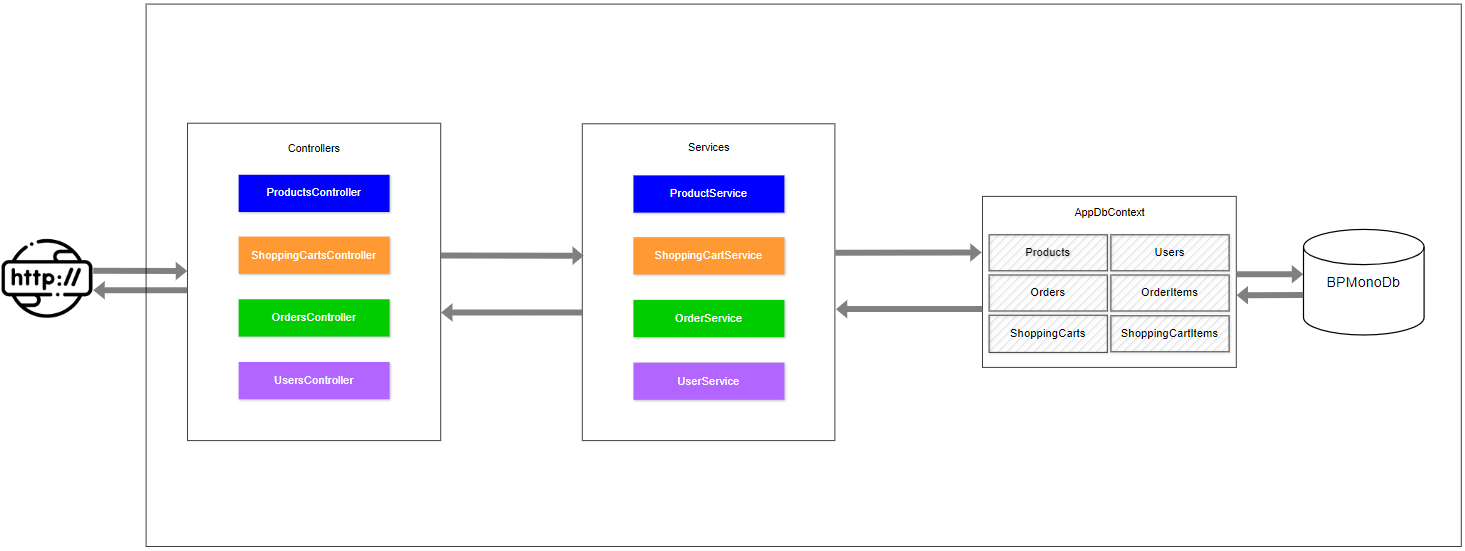
\includegraphics[width=1\textwidth]{BPMono.png}
	\caption[Voorstelling van de monolithische architectuur voor de PoC.]{\label{fig:BPMono}Voorstelling van de monolithische architectuur voor de PoC.\linebreak}
\end{figure}

De projectstructuur bevat verschillende mappen die de lagen logisch scheiden:

\begin{itemize}
	\item \textbf{Auth} - Bevat de logica voor authenticatie, waaronder een JWT-token provider voor het genereren van tokens en een wachtwoord-hasher om wachtwoorden veilig op te slaan.
	\item \textbf{Controllers} – Definiëren API-endpoints die inkomende HTTP-verzoeken van de client afhandelen en doorsturen naar de correcte services.
	\item \textbf{Data} - Omvat de AppDbContext klasse voor de database via Entity Framework Core en methodes voor het seeden van data.
	\item \textbf{Models} – Bevat domeinmodellen die de database-entiteiten representeren.
	\item \textbf{DTOs} – Data Transfer Objects die worden gebruikt om data uit te wisselen tussen de client en de server. 
	\item \textbf{Profiles} - Bevat AutoMapper-profielen die verantwoordelijk zijn voor het automatisch mappen van domeinmodellen naar DTO's en omgekeerd.
	\item \textbf{Services} – Implementeren van businesslogica en interacties met de database.
\end{itemize}

\subsection{Productbeheer}

Het productbeheer is een belangrijk onderdeel van de applicatie. Zonder producten kan de winkelwagen niets bevatten en kan er geen bestelling worden geplaatst. Hieronder volgt een voorbeeld van hoe producten beheerd worden binnen de monolithische architectuur. De \texttt{ProductsController} bevat endpoints voor CRUD-operaties, die dan gebruikmaken van de \texttt{ProductService}.

\medskip
Het eerste fragment toont het \texttt{Product}-model. Dit model representeert de structuur van een product zoals die in de database wordt opgeslagen. Elk product heeft een unieke ID, een naam en een prijs. De attributen zijn geannoteerd met data-anotaties voor validatie en database-constraints.
\medskip

\begin{lstlisting}[style=mystyleA, caption=Product.cs, label=lst:MonoProductModel]
public class Product
{
	[Key]
	[Required]
	public int Id { get; set; }
	
	[Required]
	public string Name { get; set; }
	
	[Required]
	public double Price { get; set; }
}
\end{lstlisting}

\medskip
De \texttt{ProductsController} bevat de API-endpoints waarmee de client producten kan opvragen. In het onderstaande fragment is het GET-endpoint weergegeven dat alle producten ophaalt. Dependency injection wordt gebruikt om de service en mapper te injecteren. De producten worden via de service opgehaald uit de database, en vervolgens gemapt naar \texttt{ProductReadDto}-objecten met AutoMapper.
\medskip

\begin{lstlisting}[style=mystyleA, caption=ProductsController.cs (fragment), label=lst:MonoProductsController]
[HttpGet]
public async Task<ActionResult<List<ProductReadDto>>> GetProducts()
{
	Console.WriteLine("--> Getting all products...");
	var products = await _service.GetAllProducts();
	if (products == null)
		return NotFound("No products found");
	return Ok(_mapper.Map<List<ProductReadDto>>(products));
}
\end{lstlisting}

\medskip
Tot slot wordt hieronder de implementatie van de \texttt{ProductService} weergegeven. Deze service maakt gebruik van Entity Framework Core om via de \texttt{AppDbContext} alle producten op te halen uit de database.
\medskip

\begin{lstlisting}[style=mystyleA, caption=ProductService.cs (fragment), label=lst:MonoProductService]
public async Task<List<Product>> GetAllProducts()
{
	return await _context.Products.ToListAsync();
}
\end{lstlisting}

\subsection{Winkelwagen}

Gebruikers kunnen met de winkelwagen producten bijhouden voordat deze in een bestelling worden omgezet.

\medskip
Het \texttt{ShoppingCart}-model stelt een winkelwagen voor die gekoppeld is aan een gebruiker via een \texttt{UserId}. Elke winkelwagen bevat een verzameling \texttt{ShoppingCartItem}-objecten, die de producten in de winkelwagen voorstellen.
\medskip

\begin{lstlisting}[style=mystyleA, caption=ShoppingCart.cs, label=lst:MonoShoppingCartModel]
public class ShoppingCart
{
	[Key]
	[Required]
	public int Id { get; set; }
	
	[Required]
	public int UserId { get; set; }
	
	public IEnumerable<ShoppingCartItem> Items { get; set; }
}
\end{lstlisting}

\medskip
Het \texttt{ShoppingCartItem}-model vormt de link tussen de producten en een gebruikers winkelwagen. Elk item verwijst naar zowel een \texttt{ShoppingCart} als een \texttt{Product}. Dit model maakt het mogelijk om meerdere producten aan één winkelwagen toe te voegen.
\medskip

\begin{lstlisting}[style=mystyleA, caption=ShoppingCartItem.cs, label=lst:MonoShoppingCartItemModel]
public class ShoppingCartItem
{
	[Key]
	[Required]
	public int Id { get; set; }
	
	[Required]
	public int ShoppingCartId { get; set; }
	
	[Required]
	public int ProductId { get; set; }
	
	[ForeignKey("ShoppingCartId")]
	public ShoppingCart ShoppingCart { get; set; }
	
	[ForeignKey("ProductId")]
	public Product Product { get; set; }
}
\end{lstlisting}

\medskip
De \texttt{ShoppingCartsController} bevat naast een GET-endpoint ook een PUT-endpoint om een product toe te voegen aan de winkelwagen van de ingelogde gebruiker. De \texttt{UserId} wordt uit de JWT-token van de gebruiker gehaald.
\medskip

\begin{lstlisting}[style=mystyleA, caption=ShoppingCartsController.cs (fragment), label=lst:MonoShoppingCartController]
[HttpPut("{productId}")]
public async Task<ActionResult> AddProductToCart(int productId)
{
	Console.WriteLine("--> Adding a product...");
	var userIdClaim = User.FindFirst(ClaimTypes.NameIdentifier)?.Value;
	if (string.IsNullOrEmpty(userIdClaim) || !int.TryParse(userIdClaim, out int userId))
		return Unauthorized("UserId kon niet worden bepaald uit JWT token");
	
	try
	{
		await _shoppingCartService.AddProductToCart(userId, productId);
		return Ok($"Product {productId} added to cart for user {userId}");
	}
	catch (Exception ex)
	{
		return BadRequest($"Failed to add product {productId} to cart of user {userId}: {ex.Message}");
	}
}
\end{lstlisting}

\medskip
De methode uit de \texttt{ShoppingCartService} bevat de logica om een product toe te voegen aan de winkelwagen van een specifieke gebruiker. Indien de winkelwagen nog niet bestaat voor de gebruiker, wordt er een nieuwe aangemaakt. Vervolgens wordt er een \texttt{ShoppingCartItem} toegevoegd met een verwijzing naar het product.
\medskip

\begin{lstlisting}[style=mystyleA, caption=ShoppingCartService.cs (fragment), label=lst:MonoShoppingCartService]
public async Task AddProductToCart(int userId, int productId)
{
	if (!await _context.Products.AnyAsync(p => p.Id == productId))
	throw new Exception($"No product found with id {productId}");
	
	var cart = await GetCart(userId);
	if (cart == null)
	{
		cart = new ShoppingCart { UserId = userId };
		_context.ShoppingCarts.Add(cart);
		await _context.SaveChangesAsync();
	}
	
	var cartItem = new ShoppingCartItem
	{
		ShoppingCartId = cart.Id,
		ProductId = productId
	};
	_context.ShoppingCartItems.Add(cartItem);
	await _context.SaveChangesAsync();
}
\end{lstlisting}

\subsection{Bestellingen}

Wanneer een gebruiker beslist om de producten in de winkelwagen te bestellen, wordt er een bestelling aangemaakt. Deze bestelling bevat de producten uit de winkelwagen, berekent het totaalbedrag en slaat de bestelling op in de database.

\medskip
Het \texttt{Order}-model stelt een bestelling voor die gekoppeld is aan een gebruiker via een \texttt{UserId}. Elke bestelling bevat een lijst van \texttt{OrderItem}-objecten, samen met de totale prijs en een status dat de progressie van de bestelling bijhoudt.
\medskip

\begin{lstlisting}[style=mystyleA, caption=Order.cs, label=lst:MonoOrderModel]
public class Order
{
	[Key]
	[Required]
	public int Id { get; set; }
	
	[Required]
	public int UserId { get; set; }
	
	public List<OrderItem> Items { get; set; }
	
	[Required]
	public double TotalPrice { get; set; }
	
	[Required]
	public string Status { get; set; }
}
\end{lstlisting}

\medskip
Het \texttt{OrderItem}-model bevat de details van elk besteld product, zoals de naam, prijs en bijbehorend order-ID.
\medskip

\begin{lstlisting}[style=mystyleA, caption=OrderItem.cs, label=lst:MonoOrderItemModel]
public class OrderItem
{
	[Key]
	[Required]
	public int Id { get; set; }
	
	[Required]
	public int ProductId { get; set; }
	
	[Required]
	public string Name { get; set; }
	
	[Required]
	public double Price { get; set; }
	
	[Required]
	public int OrderId { get; set; }
	
	[ForeignKey("OrderId")]
	public Order Order { get; set; }
}
\end{lstlisting}

\medskip
De \texttt{OrdersController} bevat een POST-endpoint om een bestelling te plaatsen. Allereerst wordt er gecontroleerd of de gebruiker correct geïdentificeerd is via de JWT-token. Daarna wordt de winkelwagen opgehaald en omgezet in een orderobject met AutoMapper. Vervolgens wordt de totaalprijs berekend, de order opgeslagen en de winkelwagen verwijderd.
\medskip

\begin{lstlisting}[style=mystyleA, caption=OrdersController.cs (fragment), label=lst:MonoOrdersController]
[HttpPost]
public async Task<ActionResult<OrderReadDto>> CreateOrder()
{
	try
	{
		Console.WriteLine("--> Placing an order...");
		var userIdClaim = User.FindFirst(ClaimTypes.NameIdentifier)?.Value;
		if (string.IsNullOrEmpty(userIdClaim) || !int.TryParse(userIdClaim, out int userId))
		return Unauthorized("UserId kon niet worden bepaald uit JWT token");
		
		var cart = await _shoppingCartService.GetCart(userId);
		if (cart is null) return NotFound($"ShoppingCart not found for user {userId}");
		var cartDto = _mapper.Map<ShoppingCartReadDto>(cart);
		var orderToPlace = _mapper.Map<Order>(cartDto);
		orderToPlace.Status = "Verwerking";
		orderToPlace.TotalPrice = orderToPlace.Items.Sum(i => i.Price);
		
		await _orderService.PlaceOrder(orderToPlace);
		await _shoppingCartService.RemoveCartOfUser(userId);
		
		var orderReadDto = _mapper.Map<OrderReadDto>(orderToPlace);
		return CreatedAtRoute(nameof(GetOrderById), new { OrderId = orderReadDto.Id }, orderReadDto);
	}
	catch (Exception ex)
	{
		return BadRequest(ex.Message);
	}
}
\end{lstlisting}

\medskip
De logica voor het effectief plaatsen van een bestelling bevindt zich in de \texttt{OrderService}, die de order opslaat in de database.
\medskip

\begin{lstlisting}[style=mystyleA, caption=OrderService.cs (fragment), label=lst:MonoOrderService]
public async Task PlaceOrder(Order orderToPlace)
{
	_context.Orders.Add(orderToPlace);
	await _context.SaveChangesAsync();
}
\end{lstlisting}

\medskip
Tot slot wordt de winkelwagen verwijderd via de \texttt{ShoppingCartService}, om te voorkomen dat reeds bestelde producten nog in de winkelwagen blijven.
\medskip

\begin{lstlisting}[style=mystyleA, caption=RemoveCartOfUser in ShoppingCartService.cs, label=lst:MonoRemoveCart]
public async Task RemoveCartOfUser(int userId)
{
	var cart = await _context.ShoppingCarts.FirstOrDefaultAsync(c => c.UserId == userId);
	if (cart != null)
	{
		_context.ShoppingCarts.Remove(cart);
		await _context.SaveChangesAsync();
	}
}
\end{lstlisting}

%% \subsection{Gebruikers}

\section{Implementatie van de microservices-applicatie}

In deze sectie wordt de implementatie van de microservices-applicatie nader bekeken. De monolithische versie bundelde alles in één enkele applicatie, hier wordt elke service verantwoordelijk voor zijn eigen functionaliteiten en databank. Elke microservice wordt afzonderlijk ontworpen, gecontaineriseerd en gedeployed binnen een Kubernetes-cluster.

\subsection{Architectuur en projectstructuur}

De microservices-applicatie bestaat uit vier services: \texttt{ProductService}, \texttt{ShoppingCartService}, \texttt{OrderService} en \texttt{UserService}. Elke van deze services communiceert via een RESTful API en is gecontaineriseerd met Docker en Kubernetes.

\begin{figure}[H]
	\centering
	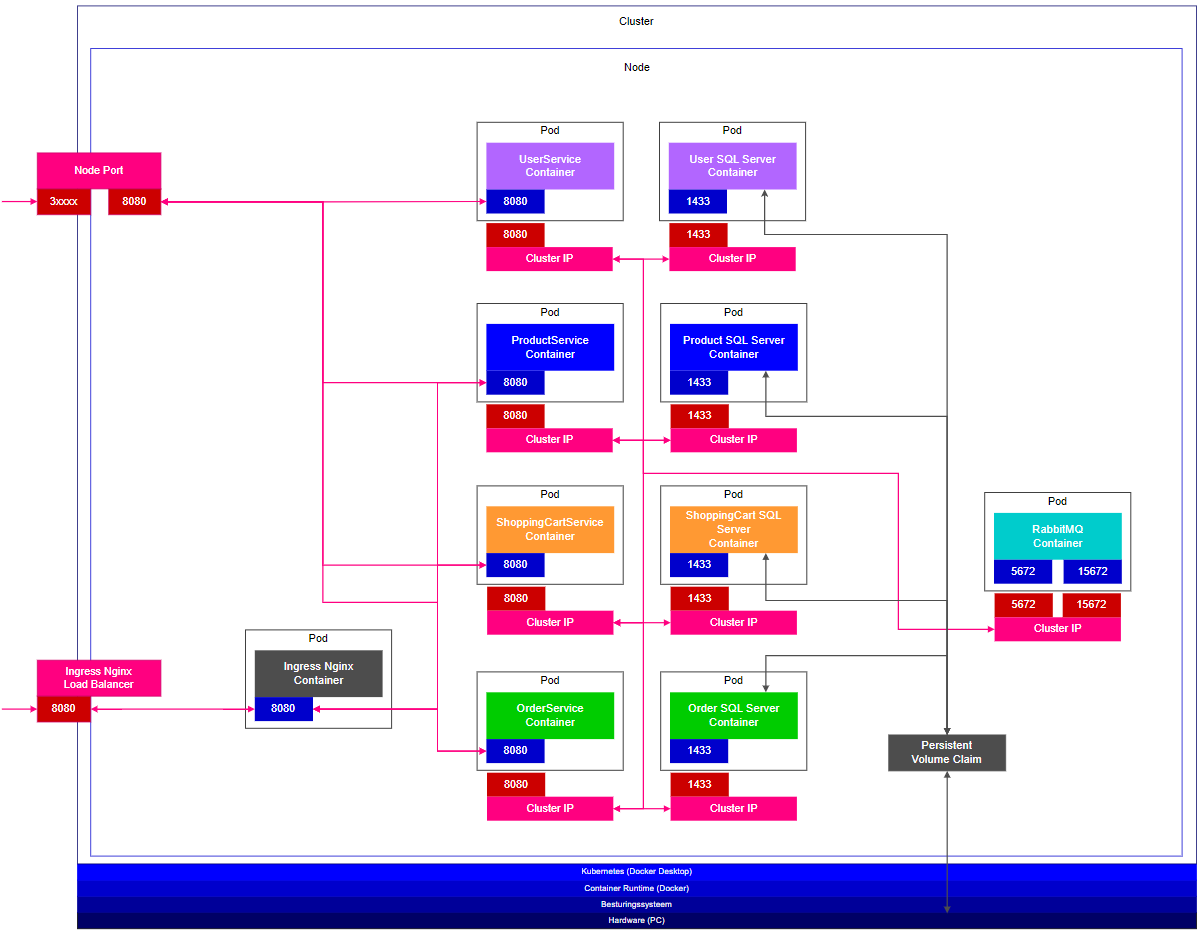
\includegraphics[width=1\textwidth]{BPMicro.png}
	\caption[Voorstelling van de microservices-architectuur voor de PoC.]{\label{fig:BPMicro}Voorstelling van de microservices-architectuur voor de PoC.\linebreak}
\end{figure}

De projectstructuur van de microservices is grotendeels gelijk aan die van de monolithische applicatie. Behalve de \texttt{UserService}, die is ontwikkeld in JavaScript en het Express framework. Deze keuze werd gemaakt om de flexibiliteit in technologiekeuze te demonstreren, zoals eerder besproken in de sectie over \hyperref[sec:flexibiliteit_technologiekeuze]{flexibiliteit in technologiekeuze}.

Daarnaast bevatten de \texttt{ShoppingCartService} en de \texttt{OrderService} een aantal extra mappen voor het afhandelen van asynchrone communicatie. Deze mappen bevatten de configuratie van RabbitMQ, event-handlers en data transfer objecten specifiek voor de asynchrone communicatie tussen beide services.

\subsection{Interservice communicatie}

In een microservices-architectuur is de communicatie tussen verschillende services een essentieel onderdeel om een goed functionerende applicatie te ontwerpen. Deze communicatie kan op twee manieren verlopen: synchroon of asynchroon. In volgend hoofdstuk worden beide vormen van communicatie getoond aan de hand van de implementatie.

\subsubsection{Synchrone communicatie}

Binnen de microservices versie van de applicatie wordt synchrone communicatie bijvoorbeeld gebruikt tussen de \texttt{ProductService} en de \texttt{ShoppingCartService}. Wanneer de \texttt{ShoppingCartService} een product wil toevoegen aan een winkelwagen, wordt eerst een HTTP-request verstuurd naar de \texttt{ProductService} om te controleren of het product bestaat. Pas nadat de \texttt{ShoppingCartService} een antwoord krijgt wordt er verder gegaan. Dit zorgt er wel voor dat de 2 services afhankelijker van elkaar worden.
\medskip

\begin{lstlisting}[style=mystyleA, caption=ShoppingCartsController.cs (fragment)(Microservice), label=lst:MicroSCCPUT]
[HttpPut("{productId}")]
public async Task<ActionResult> AddProductToCart(int productId)
{
	Console.WriteLine("--> Adding a product...");
	
	var userIdHeader = Request.Headers["UserId"].FirstOrDefault();
	if (string.IsNullOrEmpty(userIdHeader))
		return BadRequest("UserId header is required");
	
	var productExists = await _productClient.DoesProductExists(productId);
	if (!productExists)
		return BadRequest($"Product with id {productId} does not exist");
	
	var response = await _repository.AddProductToCart(userId, productId);
	
	if (response)
		return Ok($"Product {productId} added to cart for user {userId}");
	else
		return BadRequest($"Failed to add product {productId} to cart for user {userId}");
}
\end{lstlisting}

\begin{lstlisting}[style=mystyleA, caption=ProductDataClient.cs (fragment)(Microservice), label=lst:MicroProductDataCl]
public async Task<bool> DoesProductExists(int productId)
{
	Console.WriteLine("--> Does product exists?");
	var response = await _httpClient.GetAsync($"{_configuration["ProductService"]}/{productId}");
	if (response.IsSuccessStatusCode)
		return true;
	return false;
}
\end{lstlisting}

\subsubsection{Asyncrhone communicatie}

Asynchrone communicatie is terug te vinden tussen de \texttt{OrderService} en de \texttt{ShoppingCartService}. Deze moeten namelijk niet wachten op een antwoord van de andere service om ver te kunnen met hun intern proces. Wanneer een bestelling wordt geplaatst, wordt er via RabbitMQ een bericht verstuurd dat een bestelling met betrekking tot een bepaalde winkelwagen is aangemaakt. De \texttt{ShoppingCartService} ontvangt dit bericht en verwijdert de desbetreffende winkelwagen.\newline

Onderstaand fragment uit de \texttt{OrdersController} toont het POST-endpoint die gebruikt wordt wanneer een gebruiker zijn bestelling wil plaatsen. Hier zal eerst een synchroon request uitgevoerd worden naar de \texttt{ShoppingCartService} om de gebruikers zijn/haar winkelwagen op te halen. Na het aanmaken van de bestelling wordt een asynchoon bericht verstuurd via de \texttt{MessageBusClient}.\medskip

\begin{lstlisting}[style=mystyleA, caption=OrdersController.cs (fragment)(Microservice), label=lst:MicroOrdersC]
[HttpPost]
public async Task<ActionResult<OrderReadDto>> CreateOrder()
{
	Console.WriteLine("--> Placing an order...");
	try
	{
		// Get the user ID from the logged-in user
		var userIdHeader = Request.Headers["UserId"].FirstOrDefault();
		if (string.IsNullOrEmpty(userIdHeader))
			return BadRequest("UserId header is required");
		if (!int.TryParse(userIdHeader, out int userId))
			return BadRequest("UserId header must be a valid integer");
		
		var shoppingCartDto = await _dataClient.GetShoppingCartContent(userId);
		var orderToPlace = _mapper.Map<Order>(shoppingCartDto);
		orderToPlace.Status = "Verwerking";
		orderToPlace.TotalPrice = orderToPlace.Items.Sum(i => i.Price);
		
		await _repository.PlaceOrder(orderToPlace);
		
		var orderReadDto = _mapper.Map<OrderReadDto>(orderToPlace);
		
		// Tell the ShoppingCartService about the order
		try
		{
			var orderPublishedDto = _mapper.Map<OrderPublishedDto>(orderReadDto);
			orderPublishedDto.Event = "Order_Published";
			await _messageBusClient.PublishNewOrder(orderPublishedDto);
		}
		catch (Exception ex)
		{
			Console.WriteLine($"--> Could not send asynchronously: {ex.Message}");
		}
		
		return CreatedAtRoute(nameof(GetOrderById), new { OrderId = orderReadDto.Id }, orderReadDto);
	}
	catch (Exception ex)
	{
		return BadRequest(ex.Message);
	}
}
\end{lstlisting}

In de \texttt{MessageBusClient} wordt het bericht geformatteerd als JSON en op de RabbitMQ-messagebus geplaatst, zodat de \texttt{ShoppingCartService} het bericht kan ontvangen en de nodigde acties kan uitvoeren.\medskip

\begin{lstlisting}[style=mystyleA, caption=MessageBusClient.cs (fragment) (Microservice), label=lst:MicroMessageBusCl]
public async Task PublishNewOrder(OrderPublishedDto orderPublishedDto)
{
	var message = JsonSerializer.Serialize(orderPublishedDto);
	
	if (_channel == null || _connection == null)
	{
		throw new InvalidOperationException("RabbitMQ connection is not initialized");
	}
	
	if (_connection.IsOpen)
	{
		Console.WriteLine("--> RabbitMQ Connection Open, sending something...");
		// Put the OrderPublishedDto onto the MessageBus
		await SendMessage(message);
	}
	else
	{
		Console.WriteLine("--> RabbitMQ Connection is closed, not sending");
	}
}

private async Task SendMessage(string message)
{
	var body = Encoding.UTF8.GetBytes(message);
	
	await _channel.BasicPublishAsync(
		exchange: "trigger",
		routingKey: "",
		body: body
	);
	Console.WriteLine($"--> We have sent {message}");
}
\end{lstlisting}

In de \texttt{ShoppingCartService} wordt er geluisterd naar de message bus. Wanneer de \texttt{OrderService} via RabbitMQ een bericht verstuurt, controleert de \texttt{ShoppingCartService} of het om een geldig event gaat. Indien dit het geval is, wordt de winkelwagen van de gebruiker verwijderd.\medskip

\begin{lstlisting}[style=mystyleA, caption=MessageBusSub.cs (fragment) (Microservice), label=lst:MicroMessageBusSb]
private async void WaitForEvents()
{
	var consumer = new AsyncEventingBasicConsumer(_channel);
	
	consumer.ReceivedAsync += (model, ea) =>
	{
		Console.WriteLine("--> Event Received!");
		byte[] body = ea.Body.ToArray();
		var message = Encoding.UTF8.GetString(body);
		_eventProcessor.ProcessEvent(message);
		return Task.CompletedTask;
	};
	
	await _channel.BasicConsumeAsync(queue: _queueName, autoAck: true, consumer: consumer);
}
\end{lstlisting}

\begin{lstlisting}[style=mystyleA, caption=EventProcessor.cs (fragment) (Microservice), label=lst:MicroEventPrc]
public async Task ProcessEvent(string message)
{
	var eventType = DetermineEvent(message);
	
	switch (eventType)
	{
		case EventType.OrderPublished:
			await RemoveShoppingCart(message);
			break;
		default:
			break;
	}
}
\end{lstlisting}

\subsection{Kubernetes deployment}

Zoals eerder vermeld in \hyperref[containerisatie_orkestratie]{containerisatie en orkestratie} worden de microservices beheert via Kubernetes. Elke microservice heeft een aantal YAML-bestanden: een deployment YAML voor de deployment van de service; een NodePort YAML om de service extern toegankelijk te maken; een SQL deployment YAML voor de bijhorende database. Hieronder volgt een voorbeeld van de YAML-bestanden van de \texttt{ProductService}.\newline

Het fragment een voorbeeld van een service deployment. Hierin wordt vermeldt op welke Docker image de deployment gebasseerd moet zijn. Alsook wordt een \texttt{ClusterIP} ingesteld zodat, indien nodig, andere services deze service kunnen aanspreken via deze identifier.\medskip

\begin{lstlisting}[style=mystyleA, caption=bpproducts-depl.yaml, label=lst:BPProductsDepl]
apiVersion: apps/v1
kind: Deployment
metadata:
	name: bpproducts-depl
spec:
	replicas: 1
	selector:
		matchLabels:
			app: bpproductservice
	template:
		metadata:
			labels:
				app: bpproductservice
		spec:
			containers:
				- name: bpproductservice
  		  		  image: hogentjaspervandenbroucke/bpproductservice:latest
---
apiVersion: v1
kind: Service
metadata:
	name: bpproducts-clusterip-service
spec:
	type: ClusterIP
	selector:
		app: bpproductservice
	ports:
		- name: bpproductservice
  		  protocol: TCP
  		  port: 8080
  		  targetPort: 8080
\end{lstlisting}

Vervolgens wordt voor elke service een \texttt{NodePort} opgezet. Deze \texttt{NodePort} krijgt van Kubernetes een uniek id van 5 cijfers, startend met een 3.\medskip

\begin{lstlisting}[style=mystyleA, caption=bpproducts-np-srv.yaml, label=lst:BPProductsNP]
apiVersion: v1
kind: Service
metadata:
	name: bpproductnpservice-srv
spec:
	type: NodePort
	selector:
		app: bpproductservice
	ports:
		- name: bpproductservice
		  protocol: TCP
		  port: 8080
		  targetPort: 8080
\end{lstlisting}

Tot slot heeft elke service zijn eigen SQL Server database deployment. Naast de deployment en \texttt{ClusterIP} heeft deze YAML ook een \texttt{LoadBalancer}. Met behulp van de \texttt{LoadBalancer} kan er van buiten Kubernetes connectie gemaakt worden met de database. Om te kunnen connecteren met de databank moet er ingelogd worden met gebruikersnaam en wachtwoord. Het wachtwoord wordt in een Kubernetes Secret opgeslagen.\medskip

\begin{lstlisting}[style=mystyleA, caption=bpproducts-sql-depl.yaml, label=lst:BPProductsSQLDepl]
apiVersion: apps/v1
kind: Deployment
metadata:
	name: bpproducts-sql-depl
spec:
	replicas: 1
	selector:
		matchLabels:
			app: bpproducts-sql
	template:
		metadata:
			labels:
				app: bpproducts-sql
		spec:
			containers:
				- name: bpproducts-sql
				  image: mcr.microsoft.com/mssql/server:2019-latest
				  ports:
					- containerPort: 1433
				  env:
					- name: MSSQL_PID
					  value: "Express"
					- name: ACCEPT_EULA
					  value: "Y"
					- name: SA_PASSWORD
					  valueFrom:
						secretKeyRef:
							name: bp-products-sql
							key: SA_PASSWORD
				  volumeMounts:
					- mountPath: /var/opt/mssql/data
					  name: sqlproductsdb
			volumes:
				- name: sqlproductsdb
				  persistentVolumeClaim:
					claimName: bpproducts-sql-claim
---
apiVersion: v1
kind: Service
metadata:
	name: bpproducts-sql-clusterip-service
spec:
	type: ClusterIP
	selector:
		app: bpproducts-sql
	ports:
		- name: bpproducts-sql
		  protocol: TCP
		  port: 1433
		  targetPort: 1433
---
apiVersion: v1
kind: Service
metadata:
	name: bpproducts-sql-loadbalancer
spec:
	type: LoadBalancer
	selector:
		app: bpproducts-sql
	ports:
		- protocol: TCP
		  port: 1433
		  targetPort: 1433
\end{lstlisting}




\chapter{\IfLanguageName{dutch}{Resultaten}{Results}}%
\label{ch:resultaten}

In dit voorlaatste hoofdstuk worden de resultaten besproken die voortkomen uit het analyseren van de PoC. Eerst worden de bevindingen uit de SonarQube-analyse besproken, waarbij gekeken zal worden naar cyclomatische en cognitieve complexiteit van beide applicaties. Daarna volgen de resultaten van de JMeter testen, waarin wordt gekeken hoe de monolithische en microservices-applicatie zich gedragen onder hoge belasting.

\section{Complexiteit}

De onderstaande tabel toont de scores van de cyclomatische en cognitieve complexiteitsanalyse uitgevoerd met SonarQube (Community Edition). Deze resultaten geven een indicatie over de moeilijkheidsgraad van de code van de beide applicaties, maar zijn mogelijks niet volledig representatief voor een productieomgeving.

Cyclomatische complexiteit toont het aantal mogelijke vertakkingen in de code, terwijl cognitieve complexiteit aantoont hoe moeilijk de code is om te begrijpen. Hoe hoger de scores, hoe ingewikkelder het meestal is om de code te onderhouden of aan te passen.

\begin{table}[H]
	\centering
	\resizebox{\textwidth}{!}{
		\begin{tabular}{|l|c|c|}
			\hline
			\textbf{Services / Applicatie} & \textbf{Cyclomatische Complexiteit} & \textbf{Cognitieve Complexiteit} \\
			\hline
			ProductService        & 46 & 16 \\
			ShoppingCartService   & 102  & 31 \\
			OrderService          & 104 & 25 \\
			AuthService           & 20  & 22 \\
			\hline
			\textbf{Microservices-applicatie} & \textbf{272} & \textbf{94} \\
			\hline
			\textbf{Monolithische applicatie} & \textbf{180} & \textbf{32} \\
			\hline
		\end{tabular}
	}
	\caption{Complexiteitsanalyse per service}
\end{table}

\subsection{Microservices-applicatie}

Bij de microservices-applicatie valt op dat de complexiteit sterk varieert per service. De \texttt{OrderService} (104 cyclomatisch, 25 cognitief) en \texttt{ShoppingCartService} (102 cyclomatisch, 31 cognitief) hebben duidelijk de hoogste complexiteit. Dit komt doordat deze services verantwoordelijk zijn voor complexere logica, zoals communicatie met andere services (zowel synchroon als asynchroon) en het publiceren van events via RabbitMQ.\newline

De \texttt{ProductService} en \texttt{AuthService} zijn eenvoudiger en bevatten minder logica, wat resulteert in lagere complexiteitsscores. In totaal komt de microservices-applicatie uit op een cyclomatische complexiteit van 272 en een cognitieve complexiteit van 94, verdeeld over vier afzonderlijke services.

\subsection{Monolithische applicatie}

De monolithische applicatie heeft lagere scores: een cyclomatische complexiteit van 180 en een cognitieve complexiteit van 32. Deze lagere scores zijn te wijten aan het feit dat alle logica zich binnen één codebase bevindt, zonder interservice communicatie of infrastructuurcomplexiteit, zoals RabbitMQ. Hierdoor worden bijvoorbeeld asynchrone communicatie tussen services vermeden, wat in een microservices-architectuur extra code veroorzaakt.\newline

Hoewel de monolithische applicatie minder complex lijkt, betekent dit niet automatisch dat het eenvoudiger is om deze te onderhouden of uit te breiden. De moeilijkheden zitten bijvoorbeeld in het doorvoeren van wijzigingen zonder onverwachte bijwerkingen te veroorzaken.

\section{Schaalbaarheid}

De schaalbaarheidstesten zijn uitgevoerd op een laptop, wat automatisch inhoud dat de beschikbare rekenkracht en netwerkcapaciteit beperkt zijn ten opzicht van een productieomgeving met server- of cloudinfrastructuur. De resultaten moeten dan ook vanuit deze situatie geïnterpreteerd worden.\newline

Om de schaalbaarheid van beide applicaties realistisch te kunnen analyseren, werden vijf verschillende gebruikersflows gedefinieerd. Deze flows stellen typische acties voor die gebruikers op verschillende momenten kunnen uitvoeren.\newline

Voor de loadtesten werden verschillende gebruikersaantallen gesimuleerd: 10, 50, 100, 200, 250, 500 en 1000 gelijktijdige gebruikers. Bij elke test werd het totaal aantal gebruikers gelijk verdeeld over de vijf flows, wat neerkomt op 20\% van de gebruikers per flow.

Hieronder volgt een overzicht van de gebruikersflows:

\begin{itemize}
	\item \textbf{Flow 1}
	\begin{enumerate}
		\item Login
		\item Bekijk productenoverzicht
		\item Zoek specifiek product
		\item Voeg product toe aan winkelwagen (3x)
		\item Plaats bestelling
	\end{enumerate}
	
	\item \textbf{Flow 2}
	\begin{enumerate}
		\item Login
		\item Bekijk bestellingen
		\item Voeg toe aan winkelwagen (2x)
		\item Plaats bestelling
		\item Voeg toe aan winkelwagen (2x)
		\item Plaats bestelling
		\item Bekijk bestellingen
	\end{enumerate}
	
	\item \textbf{Flow 3}
	\begin{enumerate}
		\item Foutief inloggen (wachtwoord)
		\item Opnieuw inloggen (goed)
		\item Zoek specifiek product (foutief)
		\item Voeg product toe aan winkelwagen (1x)
		\item Voeg product toe aan winkelwagen (foutief)
		\item Bekijk winkelwagen
	\end{enumerate}
	
	\item \textbf{Flow 4}
	\begin{enumerate}
		\item Login
		\item Voeg product toe aan winkelwagen (4x)
		\item Bekijk productenoverzicht
		\item Plaats bestelling
		\item Voeg product toe aan winkelwagen (2x)
		\item Bekijk winkelwagen
		\item Voeg product toe aan winkelwagen (1x)
		\item Plaats bestelling
		\item Bekijk bestellingen
	\end{enumerate}
	
	\item \textbf{Flow 5}
	\begin{enumerate}
		\item Registreren nieuwe gebruiker
		\item Foutief inloggen (gebruikersnaam)
		\item Opnieuw inloggen (goed)
		\item Bekijk productenoverzicht
		\item Voeg product toe aan winkelwagen (2x)
		\item Bekijk bestellingen
		\item Plaats bestelling
	\end{enumerate}
\end{itemize}

Bij de analyse van bovenstaande flows werd voornamelijk gekeken naar de gemiddelde responstijd (in milliseconden), het foutpercentage, de hoeveelheid requests die verwerkt worden per seconde (throughput) en de hoeveelheid ontvangen en verzonden kilobytes per seconde.

\subsection{Monolithische applicatie}

De tabel hieronder toont de resultaten van de JMeter-loadtesten voor de monolithische applicatie, waarbij elke gebruiker één van de vijf vooraf gedefinieerde gebruikersflows doorliep.

\begin{table}[H]
	\centering
	\resizebox{\textwidth}{!}{
		\begin{tabular}{|l|c|c|c|c|c|}
			\hline
			\textbf{Gebruikers} & \textbf{Gem. Responstijd (ms)} & \textbf{Foutpercentage \%} & \textbf{Throughput} & \textbf{Ontvangen KB/sec} & \textbf{Verzonden KB/sec} \\
			\hline
			10 & 49 & 9.30\% & 3.8/sec & 1.62 & 1.55 \\
			\hline
			50 & 67 & 9.30\% & 18.8/sec & 17.08 & 7.65 \\
			\hline
			100 & 222 & 9.30\% & 34.3/sec & 50.49 & 13.95 \\
			\hline
			200 & 786 & 9.30\% & 55.4/sec & 144.14 & 22.61 \\
			\hline
			250 & 1586 & 9.30\% & 53.1/sec & 170.86 & 21.71 \\
			\hline
			500 & 4826 & 9.30\% & 59.4/sec & 347.27 & 24.30 \\
			\hline
			1000 & 10675 & 35.57\% & 59.7/sec & 507.67 & 22.79 \\
			\hline
		\end{tabular}
	}
	\caption{Overzicht van JMeter-resultaten voor de monolithische applicatie.}
\end{table}

De bovenstaande resultaten van de JMeter-loadtesten tonen aan dat de prestatie van de monolithische applicatie bij toenemende gebruikersaantallen geleidelijk vermindert. De applicatie blijft relatief stabiel tot ongeveer 200 gelijktijdige gebruikers, met een foutpercentage van 9.30\% en een aanvaardbare responstijd. Echter naarmate het aantal gebruikers toeneemt, stijgt de gemiddelde responstijd. Bij 500 gebruikers bedraagt deze al meer dan 4 seconden, en bij 1000 gebruikers loopt deze op tot meer dan 10 seconden. Tegelijkertijd stijgt het foutpercentage bij 1000 gebruikers tot 35.57\%, wat kan wijzen op een overbelasting.

De throughput vertoont in het algemeen een stijgende trend, met een toename van 3.8/sec bij 10 gebruikers tot 59.7/sec bij 1000 gebruikers. Deze hogere throughput gaat echter wel gepaard met een verhoogd foutpercentage, wat erop wijst dat veel requests wel worden ontvangen maar niet altijd correct worden verwerkt.

\subsection{Microservices-applicatie}

De onderstaande tabel toont de JMeter-resultaten voor de microservices-applicatie.

\begin{table}[H]
	\centering
	\resizebox{\textwidth}{!}{
		\begin{tabular}{|l|c|c|c|c|c|}
			\hline
			\textbf{Gebruikers} & \textbf{Gem. Responstijd (ms)} & \textbf{Foutpercentage \%} & \textbf{Throughput} & \textbf{Ontvangen KB/sec} & \textbf{Verzonden KB/sec} \\
			\hline
			10 & 30 & 9.30\% & 3.8/sec & 1.87 & 1.33 \\
			\hline
			50 & 248 & 9.30\% & 17.2/sec & 19.21 & 6.02 \\
			\hline
			100 & 757 & 9.30\% & 29.2/sec & 54.75 & 10.27 \\
			\hline
			200 & 4835 & 10.70\% & 24.0/sec & 55.75 & 8.41 \\
			\hline
			250 & 7173 & 13.44\% & 21.7/sec & 58.42 & 7.60 \\
			\hline
			500 & 14678 & 16.21\% & 23.0/sec & 120.11 & 8.04 \\
			\hline
			1000 & 10675 & 54.23\% & 54.1/sec & 193.97 & 16.33 \\
			\hline
		\end{tabular}
	}
	\caption{Overzicht van JMeter-resultaten voor de microservices-applicatie.}
\end{table}

De resultaten tonen dat bij een lage tot matige belasting (10 tot 100 gelijktijdige gebruikers) de responstijden relatief laag blijven, met een foutpercentage van 9.30\%. Vanaf 200 gebruikers nemen de responstijden echter fors toe, namelijk tot een gemiddelde van 4.8 seconden. Bij 500 gebruikers stijgt dit zelfs tot ruim 14 seconden. Wat opvalt bij het foutpercentage is dat dit gelijklopend is t.e.m. 100 gebruikers, maar daarna gestaag toeneemd tot 16.21\% bij 500 gebruikers en zelfs tot 54.23\% bij 1000 gebruikers.

De throughput bij de microservices applicatie vertoont wisselende resultaten. Tussen de 10 en 100 gebruikers stijgt de throughput van 3.8 naar 29.2 requests per seconde. Dit wijst erop dat de applicatie efficiënt werkt wanneer de belasting laag is. Echter, vanaf 200 gebruikers daalt de throughput. Hieruit kan afgeleid worden dat de applicatie niet alle inkomende request even efficiënt kan verwerken, mogelijks door de toename in communicatie via HTTP en RabbitMQ.

Bij 1000 gelijktijdige gebruikers stijgt de throughput naar 54.1/sec, wat op het eerste zicht positief lijkt. Maar deze enorme stijging gaat ook gepaard met een zeer hoog foutpercentage (54.23\%). Dit toont aan dat een groot deel van de inkomende request niet afgehandeld kunnen worden.

%% TODO: In dit hoofstuk geef je een korte toelichting over hoe je te werk bent
%% gegaan. Verdeel je onderzoek in grote fasen, en licht in elke fase toe wat
%% de doelstelling was, welke deliverables daar uit gekomen zijn, en welke
%% onderzoeksmethoden je daarbij toegepast hebt. Verantwoord waarom je
%% op deze manier te werk gegaan bent.
%% 
%% Voorbeelden van zulke fasen zijn: literatuurstudie, opstellen van een
%% requirements-analyse, opstellen long-list (bij vergelijkende studie),
%% selectie van geschikte tools (bij vergelijkende studie, "short-list"),
%% opzetten testopstelling/PoC, uitvoeren testen en verzamelen
%% van resultaten, analyse van resultaten, ...
%%
%% !!!!! LET OP !!!!!
%%
%% Het is uitdrukkelijk NIET de bedoeling dat je het grootste deel van de corpus
%% van je bachelorproef in dit hoofstuk verwerkt! Dit hoofdstuk is eerder een
%% kort overzicht van je plan van aanpak.
%%
%% Maak voor elke fase (behalve het literatuuronderzoek) een NIEUW HOOFDSTUK aan
%% en geef het een gepaste titel.

